\section{Practical Algorithm: MeLU for Cold-Start Recommendation}

Recommendation is one of the most important services to Internet giants like TikTok, Taobao, etc. Where to put clients' advertisement to achieve the best efficiency and how to deliver end user their probably favoured products is of vital importance. Nowadays, with the thriving of artificial intelligence and ML algorithms, industries tend to utilize machine learning approach to support recommendation service. Cold start problems, however, is a critical problems that needs to be addressed for ML-based recommendation systems. When the number of user is still small, how to learn quickly and  provide recommendations accurately based on the statistics given. Or, when a new user come, how to quickly generate a home page of products or videos that the user may pay more attention to. Some classic algorithms like collaborative filtering might also be applied. Unlike the system based on collaborative filtering (the latter has similar ratings to the target user with other users), the proposed system only considers the products consumed by the target user.

In order to avoid user privacy issues during cold starts, many web-based systems (such as Netflix) recommend items based on minimal user information only. Netflix initially showed popular movies and TV shows to new users: we call these videos as candidate products. Then, the user selects his/her favorite video from the candidates. After that, the system will recommend some programs based on the video selected by the user. Recently, in order to improve performance, recommendations have been made using deep learning methods. However, for new users who only rated a few items, the cold start problem still exists.

To solve the cold-start problem of recommendation\cite{Dong2020MAMOMM,Lu2020MetalearningOH,Liu2020AHG,Hansen2020ContentawareNH,Li2019FromZL,Zhang2020JointPM},one can use meta-learning approach like MAML , because this is a typical few-shot learning scenario. A practical work presented by paper MeLU\cite{lee2019melu}, designs and implements a recommendation system based on MAML. 

\begin{figure}[H] 
    \centering 
    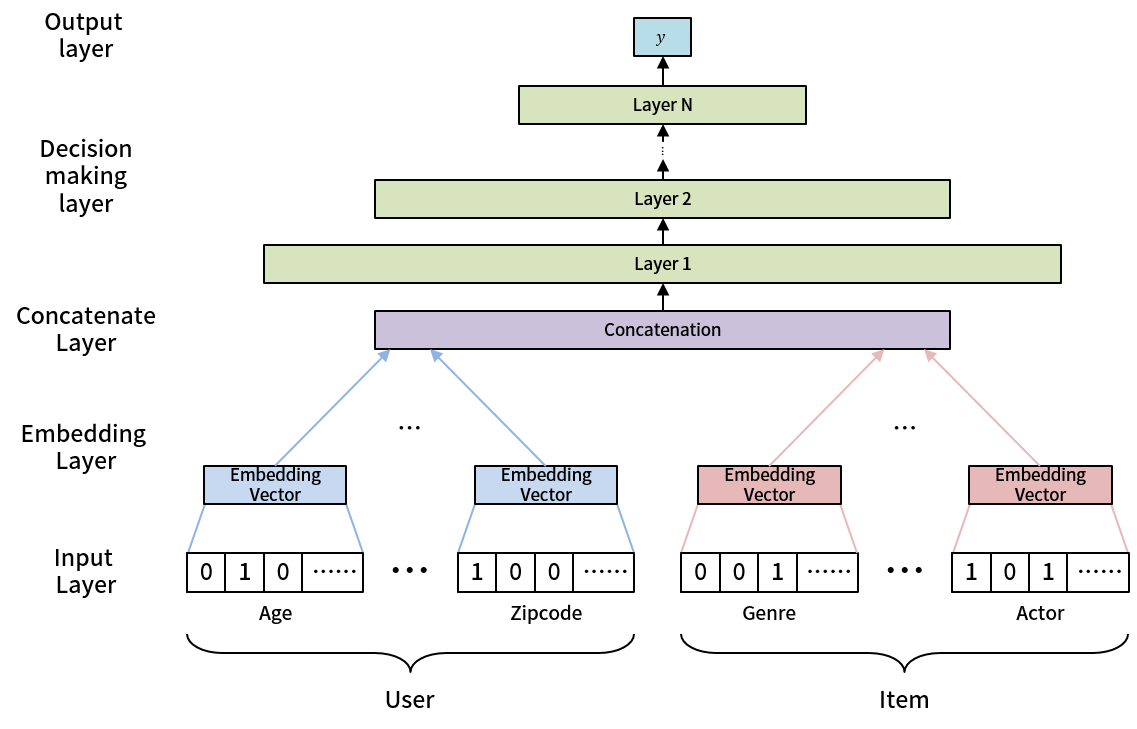
\includegraphics[width=0.7\textwidth]{image/MeLU-arch.png} 
    \caption{MeLU's User preference estimatior.}
    \label{fig:melu-estimator} 
\end{figure}

\begin{figure}[H] 
    \centering 
    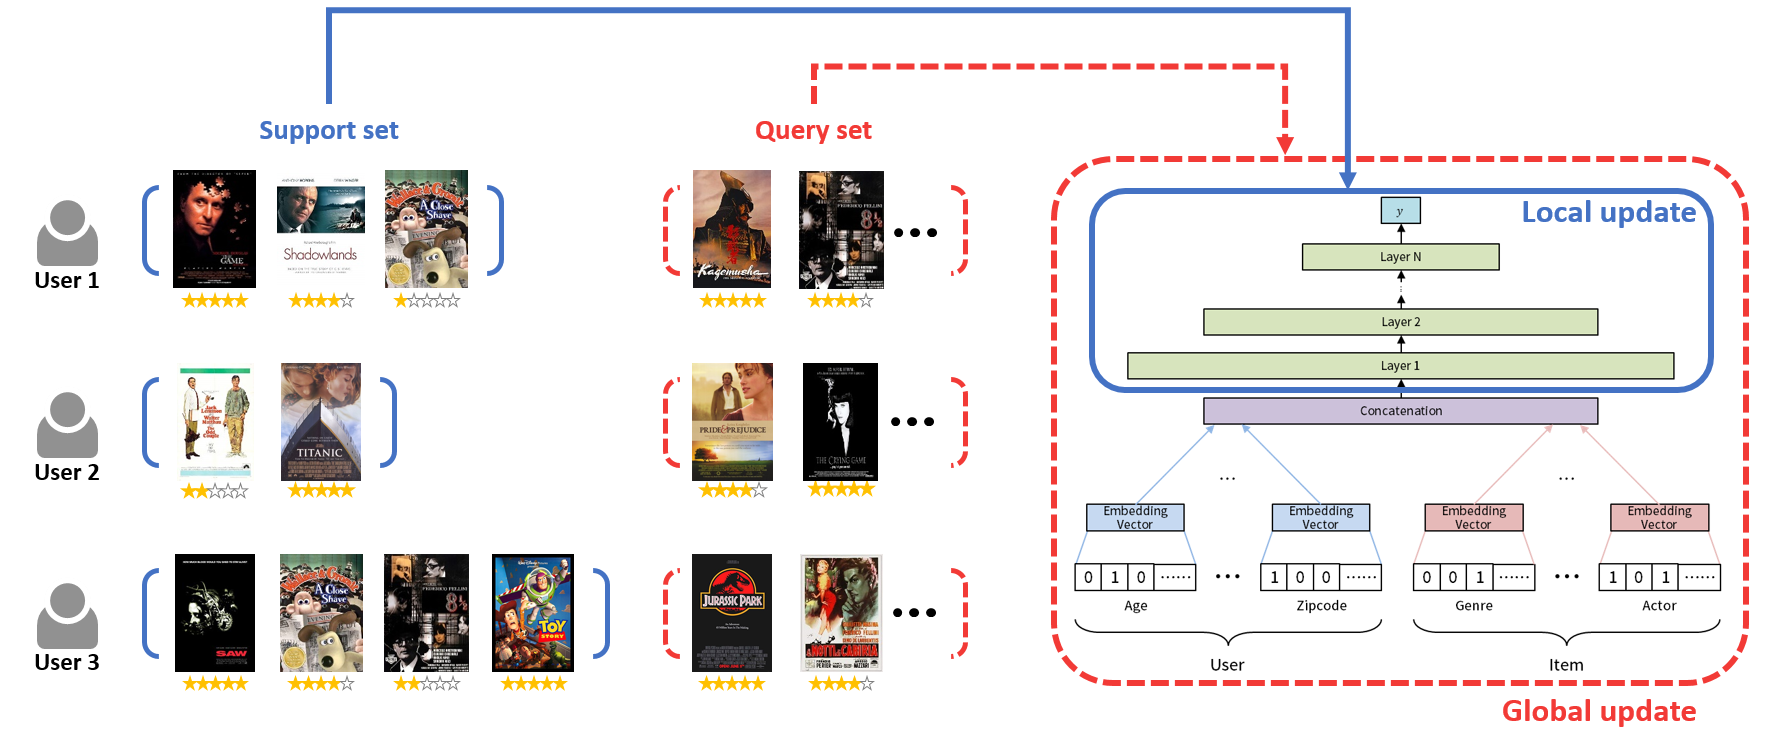
\includegraphics[width=0.7\textwidth]{image/MeLU-update.png} 
    \caption{MeLU's User preference estimatior.}
    \label{fig:melu-updates} 
\end{figure}


\subsection{MeLU's Method}
For user recommendation, MeLU first introduce a user preference estimator\ref{fig:melu-estimator} that consists of decision-making layers and output layer with user and item embeddings. MeLU model takes as input users' information and items' information, together generate an concatenated layer, and then put the concatenation into neural networks as decision making layer, and finally output a result, estimating user's preference for the item. 

Taking the standard MAML approach to meta-learn how to adapt swiftly, the model locally updates the parameters for user i in the batch by backpropagating the following loss function. 
$\mathcal{L}_i = \frac{1}{\left | H_i \right | } \sum_{j\in H_i} (y_{ij} - \hat{y}_{ij})^2 $

For the local update, each local models will update the decision making layers and output layer based on user's unique item-consumption history. While for the global update, the meta-objective, it will update both the decision making layers and output layer and embedding vectors of embedding layers, which means that our model assumes users and items do not change, only the users’ thoughts change as they interact with the items. The main different here between classic MAML and MeLU is that MeLU have assumptions for the model and update metrics, due to the specific workload characteristics. The relationship between global and local updates is illustrated in figure\ref{fig:melu-updates}. Furthermore, to improve the model performance in this scenario, MeLU do not limit the length of the item-consumption history and extend the idea of one of the most famous meta-learning algorithms, the matching network. After this optimization, the model shows good performance even when the length of the support set is not fixed across tasks.

The algorithm of MeLU is described in detail in algorithm\ref{algo-melu}.

\begin{algorithm}
    \caption{MAML for User Preference Estimator}
    \label{algo-melu}
    \begin{algorithmic}[1]
        \REQUIRE $\alpha, \beta$: step size hyperparameters
        \STATE randomly initialize $\theta_1$ (embedding vectors for the user and items)
        \STATE randomly initialize $\theta_2$ (weight matrix and bias vector for the decision-making layers)
        \WHILE {not converged}
        \STATE Sample batch of users $B \sim p(\mathcal{B})$
        \FOR {user i in B}
        \STATE set $\theta_2^i$ = $\theta_2$ 
        \STATE Evaluate $\nabla_{\theta_2^i} \mathcal{L}_i (f_{\theta_1,\theta_2^i})$
        \STATE local update $\theta_2^i \longleftarrow  \theta_2^i - \alpha\nabla_{\theta_2^i} \mathcal{L}'_i (f_{\theta_1,\theta_2^i})$
        \ENDFOR
        \STATE global update $\theta_1 \longleftarrow \theta_1 - \beta \sum_{i\in B}\nabla_{\theta_1} \mathcal{L}'_i (f_{\theta_1,\theta_2^i}) $   \\
        $\theta_2 \longleftarrow \theta_2 - \beta \sum_{i\in B}\nabla_{\theta_2} \mathcal{L}'_i (f_{\theta_1,\theta_2^i}) $  
        \ENDWHILE
    \end{algorithmic}
\end{algorithm}

MeLU also provide candidate selection strategy, that select typical evidence candidate which can help the model learn faster about users' preference for different products. 
This strategy can quickly analyze the distinguishing items of the personal preferences of new users in the system. In the model of this article, the larger the average Frobenius norm of the entire user's personalized gradient, the better the difference between user preferences. When calculating the gradient, we modify |·| to indicate the absolute value of the input to backpropagate the unit error. Although products with large gradients can be used to identify user preferences, it may be difficult to make appropriate evaluations when users do not understand the product. Therefore, we also consider the user’s understanding of the product. We assume that the more frequently the user interacts with the product, the better the user understands the product. Therefore, for each item, we use the existing full user-item pairs to calculate the gradient-based value and the popularity-based value as the average Frobenius norm and the number of interactions for each product. In order to scale the unit of two values, we normalize the value to a range from zero to one, and then assign a score to each item by multiplying the two normalized values. Finally, we define the top k items with the highest scores as commodity candidates.

The collaboration between this modified MAML algorithm, specifically for recommendation scenario, and the evidence candidate selection strategy , solve the few-shot learning problem in cold-start recommendation systems better than other similar ML/DL systems. 